\documentclass[12]{report}

\usepackage{amssymb,amsmath}

%\usepackage{refcheck}

\usepackage{graphicx}
\usepackage{amssymb}
\usepackage{mathrsfs}
\usepackage{amsmath}
\usepackage{latexsym}
\usepackage{amssymb}
\usepackage{enumerate}
\usepackage{fullpage} 
\usepackage{setspace}
\usepackage{color}
%\usepackage{ dsfont }
\usepackage{float}
\usepackage{physics}
\usepackage{hyperref}

\hypersetup{colorlinks = true}

%new math symbols taking no arguments
\newcommand\0{\mathbf{0}}
\newcommand\CC{\mathbb{C}}
\newcommand\FF{\mathbb{F}}
\newcommand\NN{\mathbb{N}}
\newcommand\QQ{\mathbb{Q}}
\newcommand\RR{\mathbb{R}}
\newcommand\ZZ{\mathbb{Z}}
\newcommand\bb{\mathbf{b}}
\newcommand\kk{\Bbbk}
\newcommand\mm{\mathfrak{m}}
\newcommand\pp{\mathfrak{p}}
\newcommand\xx{\mathbf{x}}
\newcommand\yy{\mathbf{y}}
\newcommand\GL{\mathit{GL}}
\newcommand\into{\hookrightarrow}
\newcommand\nsub{\trianglelefteq}
\newcommand\onto{\twoheadrightarrow}
\newcommand\minus{\smallsetminus}
\newcommand\goesto{\rightsquigarrow}
\newcommand\nsubneq{\vartriangleleft}

%redefined math symbols taking no arguments
\newcommand\<{\langle}
\renewcommand\>{\rangle}
\renewcommand\iff{\Leftrightarrow}
\renewcommand\phi{\varphi}
\renewcommand\implies{\Rightarrow}

%new math symbols taking arguments
\newcommand\ol[1]{{\overline{#1}}}

%redefined math symbols taking arguments
\renewcommand\mod[1]{\ (\mathrm{mod}\ #1)}

%roman font math operators
\DeclareMathOperator\aut{Aut}

%for easy 2 x 2 matrices
\newcommand\twobytwo[1]{\left[\begin{array}{@{}cc@{}}#1\end{array}\right]}

%for easy column vectors of size 2
\newcommand\tworow[1]{\left[\begin{array}{@{}c@{}}#1\end{array}\right]}

\newtheorem{theorem}{Theorem}[section]
\newtheorem{corollary}{Corollary}[theorem]
\newtheorem{lemma}[theorem]{Lemma}
\newtheorem{exercise}[theorem]{Exercise}
\newtheorem{definition}[theorem]{Definition}

\title{PHY 781: Final Project}
\date{April 28, 2019}
\author{Faris Sbahi}

\begin{document}
\maketitle

\chapter{Project 1}

Define the lattice action

\begin{align*}
S^l_E = \sum_x \{ \frac{1}{2} \chi_x^2 - \frac{\kappa}{2} \sum_{\mu} \chi_x \chi_{x + \hat{\mu}} + g \chi_x^4 \}
\end{align*}

\begin{align*}
\kappa^{-1} := 2d + \alpha \\
\alpha := (m_0a)^2
\end{align*}

\begin{align*}
\sigma &= \frac{1}{L^d}\sum_x \langle \chi^2_x \rangle\\
\chi &= \frac{1}{L^d}\sum_{x,y} \langle \chi_x \chi_y \rangle\\
F &= \frac{1}{L^d}\sum_{x,y} \langle \chi_x \chi_y \rangle \cos (2 \pi \Delta \tau / L)
\end{align*}

and furthermore

\begin{align*}
M(L) &= 	\frac{2 \sin (\pi / L)}{\sqrt{(\chi / F) - 1}}
\end{align*}


By definition,

\begin{align*}
\langle \phi(x) \phi(y)\rangle = \frac{1}{Z} \int [d \phi] e^{-S_E(\phi)} \phi(x) \phi(y)
\end{align*}

where 


\begin{align*}
Z = \int [d\phi] e^{-S_E(\phi)}
\end{align*}

\section{Exact Computation}

\subsection{$g=0$ and $\kappa \neq 0$}
\label{sec:free-exact}

We can construct $S$ as a matrix-vector product in terms of $M$

\begin{align*}
S_E^l &= \frac{1}{2}\chi_{i}M_{ij}\chi_{j}\\
M_{ij} &= - \kappa \sum_{\mu} (\delta_{i + \mu, j} + \delta_{i - \mu, j}) + \delta_{ij}
\end{align*}

where $i + \mu$ translates $i$ to all forward neighbors in $d$ dimensions i.e. $\mu = (0, \cdots , a, \cdots 0)$. Hence, $\sum_y M(x - y)M^{-1}(y-z) = \delta_{x,z}$ implies that 

\begin{align*}
\sum_y [- \kappa \sum_{\mu} (\delta_{x + \mu, y} + \delta_{x - \mu, y}) + \delta_{xy}] M^{-1}(y-z) = \delta_{x,z}
\end{align*}

In momentum space, we have

\begin{align*}
\sum_y [- \kappa \sum_{\mu} (\delta_{x + \mu, y} + \delta_{x - \mu, y}) + \delta_{xy}] M^{-1}(y-z) &\rightarrow \sum_y \int_{- \pi / a}^{\pi / a} \frac{d^d k}{(2\pi)^d} e^{ik \cdot (y - z)} \tilde{M}^{-1}(k) [- \kappa \sum_{\mu} (\delta_{x + \mu, y} + \delta_{x - \mu, y}) + \delta_{xy}]  \\
&= \int_{- \pi / a}^{\pi / a} \frac{d^d k}{(2\pi)^d} \tilde{M}^{-1}(k) [- \kappa \sum_{\mu} (e^{ik \cdot (x + \mu - z)} + e^{ik \cdot (x - \mu - z)}) + e^{ik \cdot (x - z)}] \\
&= \int_{- \pi / a}^{\pi / a} \frac{d^d k}{(2\pi)^d} \tilde{M}^{-1}(k) [- \kappa \sum_{\mu} (e^{ik \cdot \mu} + e^{-ik \cdot \mu}) + 1]e^{ik \cdot (x - z)} \\
\delta_{x,z} &\rightarrow \int_{- \pi / a}^{\pi / a} \frac{d^d k}{(2\pi)^d} e^{ik \cdot (x - z)}
\end{align*}

Therefore, we can conclude that 

\begin{align*}
	\tilde{M}^{-1}(k) [- \kappa \sum_{\mu} (e^{ik \cdot \mu} + e^{-ik \cdot \mu}) + 1] &= 1 \\
	\tilde{M}^{-1}(k) &= \frac{1}{1 - \kappa \sum_{\mu} (e^{ik \cdot \mu} + e^{-ik \cdot \mu})} \\
	&= \frac{1}{1 - 2\kappa \sum_{\mu} \cos(k \cdot \mu)}
\end{align*}

So, we can write that the momentum in the $\mu$ direction as $k_\mu := k \cdot \mu$. Note that momentum is restricted to the Brillouin zone: $|k_\mu| \leq \pi$. Because the lattice is discretized and each dimension is of size $L$, $k_\mu$ takes on values

\begin{align*}
	k_\mu = \frac{2\pi n_\mu}{L}, \qquad n_\mu \in \{0, \cdots, L - 1 \}
\end{align*}

which gives

\begin{align*}
	\tilde{M}^{-1}(k) &= \frac{1}{1 - 2\kappa \sum_{\mu} \cos(\frac{2\pi n_\mu}{L})}
\end{align*}


Now, note that

\begin{align*}
\sum_x \chi_x^2 &= \sum_x \bra{\chi}\ket{x}	\bra{x}\ket{\chi}\\
&= \sum_k \bra{\chi}\ket{k}	\bra{k}\ket{\chi}\\
\sigma &= \frac{1}{L^d}\sum_k \langle \chi^2_k \rangle\\
&=  \sum_{n_1, \cdots, n_d} \frac{1}{1 - 2\kappa \sum_{\mu} \cos(\frac{2\pi n_\mu}{L})}
\end{align*}

Furthermore, since $|\bra{k=0}\ket{x}|^2 = \frac{e^{0}}{L^d}$ 

\begin{align*}
\sum_{x,y} \chi_x \chi_y &= \frac{1}{L^d} \sum_{x, y} \bra{\chi}\ket{x}  \bra{y}\ket{\chi} \\
&= \sum_{x, y, k, k'} \bra{\chi}\ket{k}\bra{k}\ket{x}\bra{x}\ket{0}\bra{0}\ket{y} \bra{y}\ket{k'}\bra{k'}\ket{\chi} \\
&= |\bra{k=0}\ket{\chi}|^2 \\
\chi &= \langle \chi^2_{k={(0, \cdots, 0)}} \rangle \\
&= \frac{1}{1 - 2\kappa d}
\end{align*}

Finally, using $\cos(2\pi (x_0 - y_0) / L) = (e^{2\pi i (x_0 - y_0) / L} + e^{-2\pi i (x_0 - y_0) / L})/2$ where $x_0$ is the component of $x$ along the time dimension,

\begin{align*}
\sum_{x_0,y_0} \chi_x \chi_y e^{2\pi i (x_0 - y_0) / L} &= \sum_{x_0,y_0}  \bra{\chi}\ket{x_0} \bra{x_0}\ket{k = 1} \bra{k = 1}\ket{y_0} \bra{y_0}\ket{\chi} \\
\intertext{and the same follows for complex conjugate $\sum_{x_0,y_0} \chi_x \chi_y e^{-2\pi i (x_0 - y_0) / L}$. Hence, using this result and $\chi$ above, }
F &= \langle \chi^2_{k={(1, 0, \cdots, 0)}} \rangle  \\
&= \frac{1}{1 - 2\kappa [\cos(\frac{2\pi}{L}) + d-1]}
\end{align*}

Using these derived relations, we find the following results for $L = 16, g = 0, \alpha = 0.25$,

\begin{table}[H]
\label{table:exact-kappa}
\centering
\begin{tabular}{|l|l|l|l|l|}
\hline
$d$ & $\sigma$          & $\chi$             & $F$                & $M(L)$ \\ \hline
2   & 1.6021 & 17.0000 & 10.5659 & 0.5000    \\
3   & 1.3198 & 25.0000  & 15.5380 &   0.5000  \\
4   & 1.1995  &  33.0000  & 20.5101  &    0.5000 \\ \hline
\end{tabular}
\caption{Exact Computation Results for $g=0$ and $\kappa \neq 0$}
\end{table}

\subsection{$g\neq 0$ and $\kappa = 0$}
\label{sec:no-interaction-exact}

For $\kappa = 0$, we lose interaction terms. Assume $x \neq y$ and so

\begin{align*}
S^l_E &= \sum_x \{ \frac{1}{2} \chi_x^2 + g \chi_x^4 \} \\
\< \chi_x \chi_y \> &= \frac{1}{Z} \int d \chi_x d \chi_y \prod_{i \neq x, y} d \chi_i \exp(\sum_i \{ \frac{1}{2} \chi_i^2 + g \chi_i^4 \}) \chi_x \chi_y \\
&= \frac{Z_0}{Z} \Big(\int d \chi \exp(\sum_x \{ \frac{1}{2} \chi_x^2 + g \chi_x^4 \}) \chi \Big)^2 \\
\intertext{where $Z_0 := \int \prod_{i \neq x, y} d \chi_i \exp(\sum_i \{ \frac{1}{2} \chi_i^2 + g \chi_i^4 \})$}
&= 0 \tag{$e^{-S_E}$ is even and so the integrand is odd}
\end{align*}

Therefore, only $\< \chi_x^2 \>$ is nonzero amongst two-point correlations. In which case, $\sigma = \chi = F$. And in particular we have for $g= 0.1$,

\begin{align*}
\sigma &= \frac{1}{Z}\int_{-\infty}^\infty  e^{- ((1/2) x^2 + 0.1 x^4)} \\
&= 2.14971 \\
Z &= e^{- ((1/2) x^2 + 0.1 x^4)} x^2 \\
&= 1.3232 \\
\sigma &= 0.615527
\end{align*}

independent of $L$. Of course, $\chi = F$ suggests that $M(L)$ diverges (the equation for $M(L)$ gives $M(L) \rightarrow \infty$).

\section{Monte Carlo for $g=0$ or $\kappa = 0$}

\subsection{$g=0$ and $\kappa \neq 0$}

We used the Monte Carlo algorithm with 10,000 spin and regular updates. We found the following results for $L = 16, g = 0, \alpha = 0.25$.

\begin{table}[H]
\centering
\begin{tabular}{|l|l|l|l|l|}
\hline
$d$ & $\sigma$ & $\chi$ & $F$ & $M(L)$ \\ \hline
2   & 1.5984 & 16.9759 & 10.5659 & 0.5104 \\
3   & 1.3201 & 24.5100 & 15.3275 & 0.5041 \\
4   & 1.1995  &  32.8455 & 20.3969  & 0.4994 \\ \hline
\end{tabular}
\caption{Monte Carlo Results for $g=0$ and $\kappa \neq 0$}
\end{table}

which aligns closely with Table \ref{table:exact-kappa}

\subsection{$g\neq 0$ and $\kappa = 0$}

We used the Monte Carlo algorithm with 10,000 spin and regular updates. We found the following results for $L = 16, g = 0.1, \kappa = 0, \alpha = 0.25$.

\begin{table}[H]
\centering
\begin{tabular}{|l|l|l|l|l|}
\hline
$d$ & $\sigma$ & $\chi$ & $F$ & $M(L)$ \\ \hline
2   & 0.6150 & 0.6151 & 0.6151 & $\infty$ \\
3   & 0.6156 & 0.6241 & 0.6241 & $\infty$  \\
4   & 0.6155  & 0.6211 & 0.6211  & $\infty$ \\ \hline
\end{tabular}
\caption{Monte Carlo Results for $g\neq 0$ and $\kappa = 0$}
\end{table}

which aligns closely with Section \ref{sec:no-interaction-exact}.

\section{Monte Carlo for $g\neq0$ and $\kappa \neq 0$}

% TODO - add errors

We used the Monte Carlo algorithm with 10,000 spin and regular updates. We found the following results for $L = 8, g = 0.1, \alpha = -1.5$.

\begin{table}[H]
\centering
\begin{tabular}{|l|l|l|l|l|l|l|l|}
\hline
$d$ & $\sigma$ & $\delta \sigma / \sigma$ & $\chi$ & $\delta \chi / \chi$ & $F$ & $ \delta F / F$ & $M(L)$ \\ \hline
2   & 0.8295 & 0.03\% & 6.0336 & 0.02\%& 2.4549 & 0.03\% & 0.6339 \\
3   & 0.6855 & 0.02\%& 2.8406 & 0.9\% & 2.0802 & 0.03\% & 1.2659  \\
4   & 0.6562 &  0.02\% & 2.3761 & 0.05\% & 1.9910 &  0.05\% & 1.7403 \\ \hline
\end{tabular}
\caption{Monte Carlo Results for $g\neq 0$ and $\kappa = 0$}
\end{table}


\chapter{Project 2}

\section{Computing the Physical Mass}

In the symmetric massive phase, one can argue that 


\begin{align*}
\< \phi(x) \phi(x') \> &= \int d^dp \frac{Z}{p^2 + M^2_{phys}} (1 + O(p^2)) e^{ip \cdot (x-x')}	
\end{align*}

where $Z$ is the residue of the propagator. Recall from Section \ref{sec:free-exact} that

\begin{align*}
\< \phi(x) \phi(x') \> &= \int d^dp \frac{Z}{p^2 + M^2_{phys}} e^{ip \cdot (x-x')}	
\end{align*}

is the propagator for $g = 0$. Hence, the above equation says that we can consider the infinite lattice limit in the context of the free theory. So, recall from Section \ref{sec:free-exact}, that on the lattice of the free theory,

\begin{align*}
\chi &= \frac{1}{1 - 2\kappa d}	\\
F &= \frac{1}{1 - 2\kappa [\cos(\frac{2\pi}{L}) + d-1]} \\
M(L) &= \frac{2 \sin (\pi / L)}{\sqrt{(\chi / F) - 1}} \\
\end{align*}

Therefore,

\begin{align*}
M(L) &= \frac{2 \sin (\pi / L)}{\sqrt{\frac{(1 - 2\kappa d)^{-1}}{ (1 - 2\kappa [\cos(\frac{2\pi}{L}) + d-1])^{-1}} - 1}}  \\
&= 	\frac{2 \sin (\pi / L)}{\sqrt{\frac{1 - 2\kappa [\cos(\frac{2\pi}{L}) + d-1]}{1 - 2\kappa d} - 1}} \\
&= \frac{2 \sin (\pi / L)}{\sqrt{\frac{2\kappa [1 - \cos(\frac{2\pi}{L})]}{1 - 2\kappa d}}} \\
&= \frac{2 \sin (\pi / L)}{\sqrt{\frac{4\kappa \sin^2(\frac{\pi}{L})}{1 - 2\kappa d}}} \\
&= \frac{2 \sin (\pi / L)}{\frac{2\kappa^{1/2} \sin(\frac{\pi}{L})}{(1 - 2\kappa d)^{1/2}}} \\
&= \frac{(1-2\kappa d)^{1/2}}{\kappa^{1/2}} \\
&= \frac{(1-2(2d + \alpha )^{-1} d)^{1/2}}{(2d + \alpha )^{-1/2}} \\
&= \frac{(1-\frac{2d}{2d + \alpha})^{1/2}}{(2d + \alpha )^{-1/2}} \\
&= \sqrt{2d + \alpha - 2d} = M_{phys}a
\end{align*}

as desired.

                                                                                                                                                                       
\section{Computing the Lattice Spacing}

We used the Monte Carlo algorithm with 20,000 spin and regular updates. We found the following results for $d=2, g = 0.01$, and $\alpha = -0.5$.


\begin{table}[H]
\centering
\begin{tabular}{|l|l|l|l|l|}
\hline
$L$ & $M(L)$ \\ \hline
24   & 0.272 \\
32   & 0.277  \\
48   & 0.271 \\ \hline
\end{tabular}
\caption{Monte Carlo results for lattice spacing computation}
\end{table}

\begin{figure}[H]
\centering
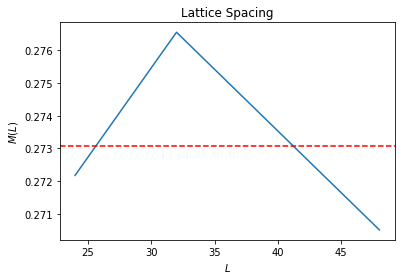
\includegraphics[width=0.7\textwidth]{lattice_spacing.png}
\caption{We see that $M(L)$ approaches a constant near $0.273$ as $L$ increases as seen by plotting $L = 24, 32, 48$.}	
\end{figure}

From the figure above, we see that $M(L) \rightarrow 0.273$ (approximately) in the infinite lattice limit. Hence, given that $M(L) \rightarrow M_{phys}a$ in the same limit, if the physical mass is $1 GeV$ then the lattice spacing is approximately $2.73 \times 10^{-10} eV$. 

\section{Renormalization}

The results of this section show that, in the large lattice limit, one can show that

\begin{align}
\label{eq:renorm}
M_{phys}a = f_0 (\alpha - \alpha_c)^\nu 
\end{align}

holds for some critical exponent $\nu$.

\subsection{$d=2$}

We used the Monte Carlo algorithm with 20,000 spin and regular updates. We found the following results for $d=2, g = 0.01$, and $L = 48$.

\begin{table}[H]
\centering
\begin{tabular}{|l|l|l|l|l|}
\hline
$\alpha$ & $M(L)$ \\ \hline
-0.55   & 0.208 \\
-0.55 & 0.193 \\
−0.57   & 0.168 \\ 
-0.58 & 0.149\\
-0.59 & 0.133 \\
-0.60 & 0.113 \\
-0.61 & 0.105 \\\hline
\end{tabular}
\caption{Monte Carlo results for $d=2$ renormalization computation}
\end{table}

Hence, for $\nu = 1$ we found that the parameters $\alpha_c = -0.669$ and $f_0 = 1.724$ minimized the least square error of Equation \ref{eq:renorm} with respect to our data.


\begin{figure}[H]
\centering
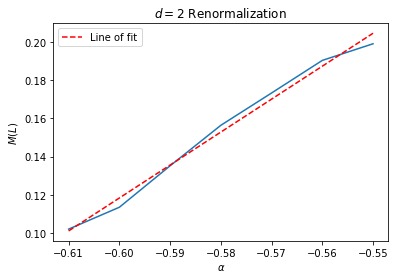
\includegraphics[width=0.7\textwidth]{renormalization_2}
\caption{$M_{phys}a$ can be given in terms of the tuning parameter roughly by $1.724(\alpha + 0.669)$}	
\end{figure}

\subsection{$d=3$}

We used the Monte Carlo algorithm with 20,000 spin and regular updates. We found the following results for $d=3, g = 0.01$, and $L = 48$.

\begin{table}[H]
\centering
\begin{tabular}{|l|l|l|l|l|}
\hline
$\alpha$ & $M(L)$ \\ \hline
-0.68   & 0.169 \\
-0.69 & 0.171 \\
-0.70   & 0.126 \\ 
-0.71 & 0.110 \\
-0.72 & 0.090 \\ \hline
\end{tabular}
\caption{Monte Carlo results for $d=3$ renormalization computation}
\end{table}

Hence, for $\nu = 0.629971$ we found that the parameters $\alpha_c = -0.669$ and $f_0 = 1.724$ minimized the least square error of Equation \ref{eq:renorm} with respect to our data.


\begin{figure}[H]
\centering
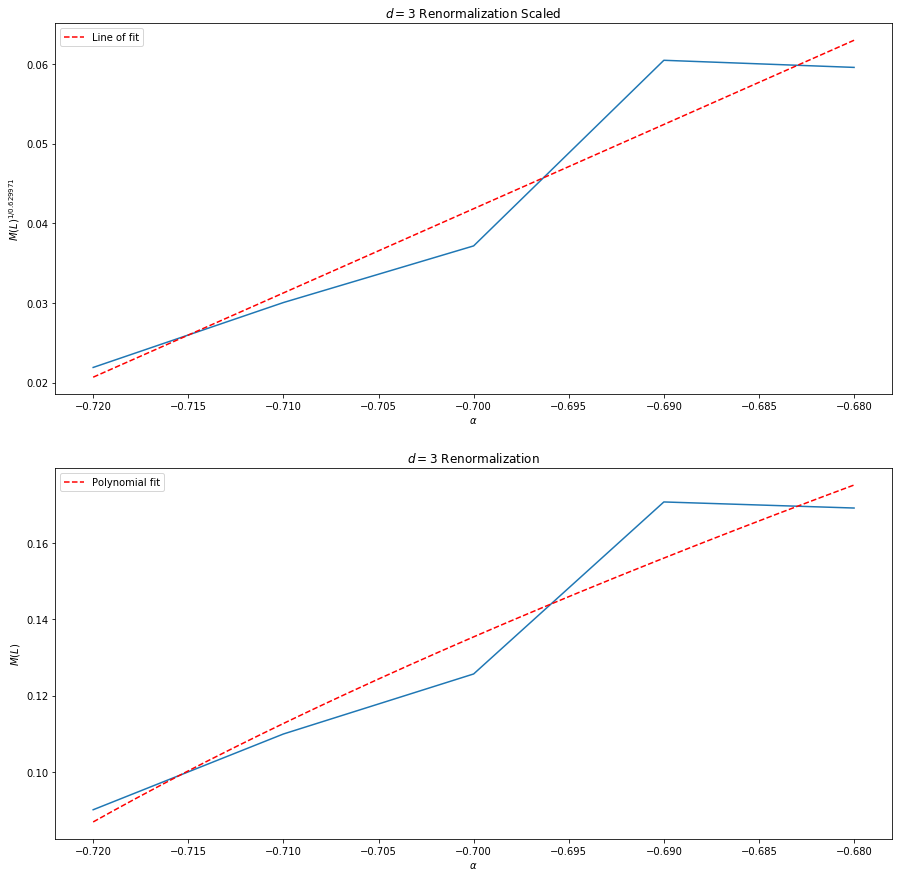
\includegraphics[width=\textwidth]{renormalization_3}
\caption{$M_{phys}a$ can be given in terms of the tuning parameter roughly by $1.036(\alpha + 0.740)^{0.629971}$}		
\end{figure}

\subsection{$d=4$}

We used the Monte Carlo algorithm with 20,000 spin and regular updates. We found the following results for $d=4, g = 0.01$, and $L = 12$.

\begin{table}[H]
\centering
\begin{tabular}{|l|l|l|l|l|}
\hline
$\alpha$ & $M(L)$ \\ \hline
-0.55   & 0.540 \\
-0.60 & 0.483 \\
-0.65   & 0.473 \\ 
-0.70 & 0.426\\
-0.75 & 0.349 \\ \hline
\end{tabular}
\caption{Monte Carlo results for $d=4$ renormalization computation}
\end{table}

Hence, for $\nu = 0.5$ we found that the parameters $\alpha_c = -0.919$ and $f_0 = 0.885$ minimized the least square error of Equation \ref{eq:renorm} with respect to our data.

\begin{figure}[H]
\centering
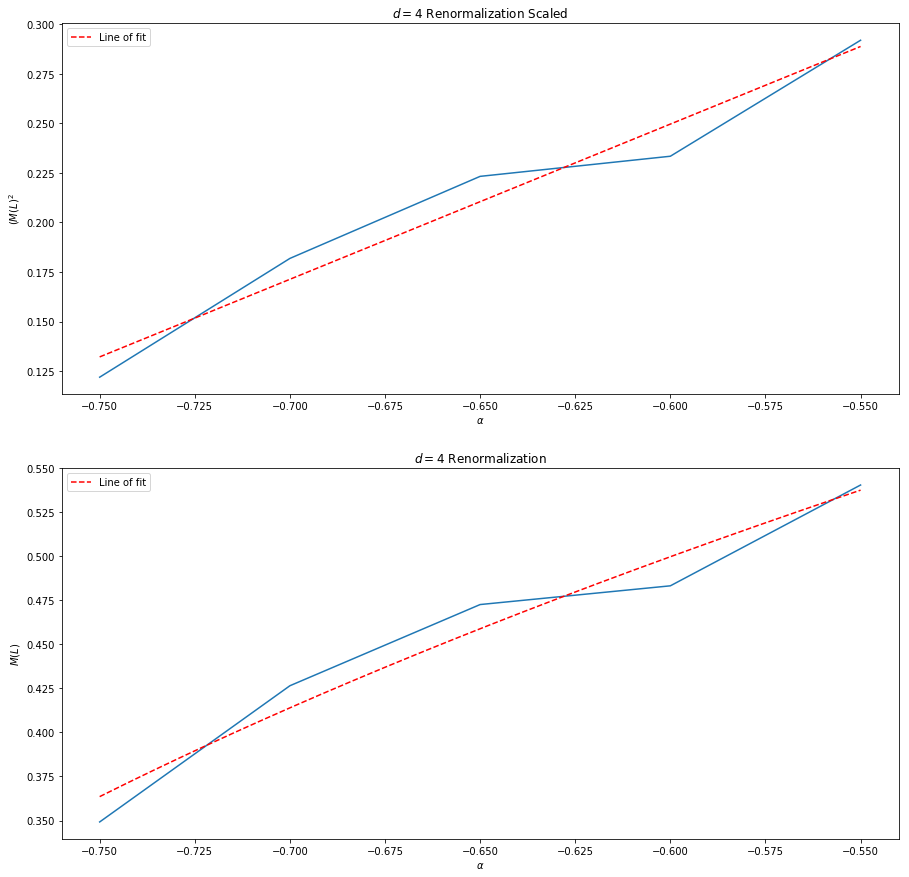
\includegraphics[width=\textwidth]{renormalization_4}
\caption{$M_{phys}a$ can be given in terms of the tuning parameter roughly by $0.885(\alpha + 0.919)^{0.5}$}		
\end{figure}

\section{Spontaneous Symmetry Breaking}

We used the Monte Carlo algorithm with 10,000 spin and regular updates. We found the following results for $d =3$ and $g = 0.01$ as we varied $\alpha$ and $L$.

\begin{table}[H]
\centering
\begin{tabular}{|l|l|l|l|l|}
\hline
$\alpha$ & $\chi(L = 16)$ & $\chi(L=24)$ & $\chi(L=32)$ & $\chi(L=48)$ \\ \hline
-0.7   & 190.31 & 221.80 & 270.33 & 248.85 \\
-0.8   & 3092.23 & 10599.55 & 25127.32 & 83722.27  \\ \hline
\end{tabular}
\caption{$\chi$ as a function of $L$ for $\alpha = -0.7, -0.8$}
\end{table}


We can see that $\chi$ diverges rapidly for $\alpha = -0.8$ whereas it remains roughly constant about $\chi = 230$ for $\alpha = -0.7$. From the previous section, we know that the critical constant for $d=3$ is given by $\alpha_c \approx 0.74$:

\begin{align}
\label{eq:sym}
	M_{phys}a \approx 1.036(\alpha + 0.740)^{0.629971}
\end{align}

We visualize the results in Figure \ref{fig:sym}.


In particular, symmetry breaking occurs at this critical point $\alpha_c \approx 0.74$. For $\alpha > \alpha_c$, $M_{phys}$ has the correct sign and so we have an ordinary scalar field theory with vacuum $\ket{\Omega}_{sym}$. However, for $\alpha < \alpha_c$, one can show that this results in $\ket{\Omega}_{sym}$ becoming an unstable equilibrium and furthermore a degeneracy in true (stable) vacua of the theory (so a choice of vacuum is necessary). This breaks the global symmetry. From Noether's Theorem, we know that a continuous global symmetry can be associated with a conserved charge. Hence, we can think of this change in the potential as we adjust the tuning parameter to fall below the critical point, as causing the symmetric vacuum which satisfies $Q\ket{\Omega}_{sym} = 0$ to become an unstable equilibrium. The true degenerate vacua of the system are charged. Hence, the results that we see are associated with the fact that the charged vacuum expectation values have a lattice size dependence.

Furthermore, Goldstone's Theorem says that spontaneous breaking of continuous global symmetries implies the existence of massless particles. Indeed, our fit equation (\ref{eq:sym}) indicates that massless particles exist at $\alpha = (m_0a)^2 = \alpha_c$.

\begin{figure}[H]
\label{fig:sym}
\centering
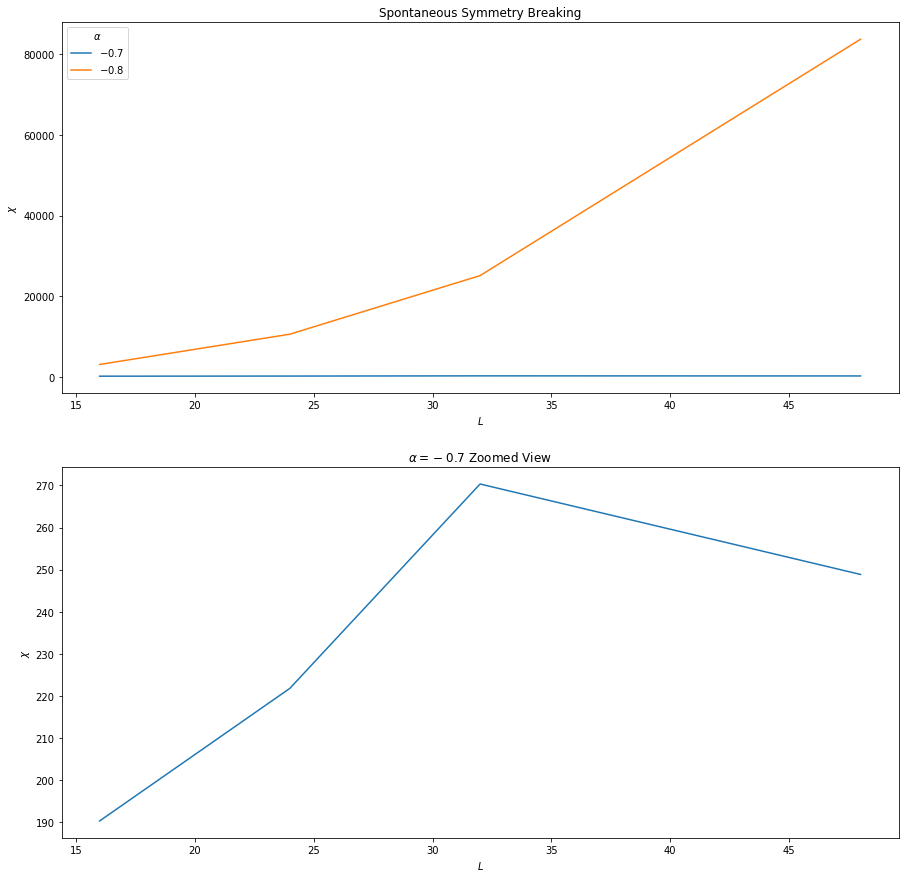
\includegraphics[width=\textwidth]{symmetry}
\caption{For $\alpha = -0.7$, $\chi$ remains roughly constant as lattice size $L$ increases. On the other hand for $\alpha = -0.8$, which is on the other side of $\alpha_c \approx 0.74$, $\chi$ diverges as $L$ increases.}		
\end{figure}

\end{document}
